\documentclass{article}

\usepackage[%
    left=0.5in,%
    right=0.5in,%
    top=0.5in,%
    bottom=0.5in,%
]{geometry}%
\usepackage{minitoc}
\usepackage{multicol}
\usepackage{graphicx}
\usepackage{fixltx2e}
\usepackage{listings}
\usepackage{color}
\usepackage{hyperref}
    \hypersetup{ colorlinks = true, linkcolor = blue }
\usepackage{blindtext}
\definecolor{lightgray}{gray}{0.9}
\graphicspath{ {./} }

\newcommand{\inlinecode}[2]{\colorbox{lightgray}{\lstinline
[language=#1]$#2$}}
\newcommand{\worddef}[1]{\hyperref[sec:reference]{\textit{#1}}}

\begin{document}

\tableofcontents

\newpage

\section{Broadcast receiver}

\begin{flushleft}
Respond to system-wide broadcast announcements
\begin{itemize}
  \item The user has not necessarily done something, but the OS / phone / another application has 
  \item The screen has turned off, the battery is low, a new SMS has arrived, the phone has booted 
  \item Can be sent by an application, or received by an application from the OS 
  \item Create the process, instantiate a BroadcastReceiver. Process doesn't have to be running continuosly, can start when needed.
\end{itemize}
\textbf{Intents} are sent to specific Activities / Services. Explicitly or implicitly via Intent filters, URI provision. \textbf{Broadcasts} are sent to anything that cares to listen. System-wide Intent broadcasts. Is declared inside \textit{Android.xml} file
  \begin{itemize}
    \item Need to specify broadcast intents we are interested in
    \item Registered and boot/install time.
  \end{itemize}
\end{flushleft}

\section{Broadcast}

\begin{flushleft}
Broadcasts are Intents
\begin{itemize}
  \item  Send an Intent to start an Activity 
  \item Send an Intent to start a Service 
  \item Send an Intent to trigger Broadcast Receivers that subscribe to that particular class of Intent 
  \begin{itemize}
    \item Can define our own Broadcast Intents 
    \item Cannot send system Intents (battery, screen etc), as the security model prevents it. Else could falsify system properties. 
    \item Again a messaging wrapper around Binder
  \end{itemize}
\end{itemize}
\end{flushleft}

\subsection{Implementing a BroadcastReceiver}

\begin{itemize}
  \item \textbf{Subclass BroadcastReciever}: Specify which Intents we are interested in receiving. Permissions permitting
  \item Implement the onReceive() method
\end{itemize}

\begin{flushleft}
Then
\begin{itemize}
  \item \textbf{Send a Message} to our application to change our behavior. Reduce the audio volume, play a sound 
  \item \textbf{Start an Activity}. Never start an Activity in response to an incoming broadcast Intent. (Would stop current activity and disrupt user experience) 
  \item \textbf{Start a Service}: A gateway to another component. How much work should a BroadcastReceiver actually do? 
  \item \textbf{Show a Notification}: Alert the user that there is something that they need to interact with at some point
\end{itemize}
\end{flushleft}

\subsection{Sticky broadcast}

\begin{flushleft}
\textbf{Non-Sticky}: If you weren’t listening at the time you’ve missed it.
\textbf{Sticky}: Intents are cached by Android
\begin{itemize}
  \item sticky intents are \textbf{deprecated}
  \item New Intents overwrite older Intents they match 
  \item Sticky broadcasts are global to the system 
  \item And because of this, performing a sticky broadcast is multiple orders of \textbf{magnitude slower} than just implementing direct calls within your own app 
  \begin{itemize}
    \item IPC for each receiver to register, IPC to the system to send it, IPC from the system back to your app to deliver it, marshalling and unmarshalling of all the data within the Intent over both IPCs 
  \end{itemize}
  \item More than that, there is \textbf{NO protection} on them, so any other application can watch your sticky broadcasts, or even send their own values back to you
\end{itemize}
No longer able to send implicit Broadcasts
\end{flushleft}

\subsection{Local Broadcasts}

\begin{itemize}
  \item Like the normal BroadcastReceiver but only supports local broadcasts (Within the application) 
  \item Data broadcast will not leave the application (No data leakage)
  \item Other applications cannot send broadcasts to our application 
  \item More efficient than sending a global broadcast (No IPC)
  \item Must register / sendBroadcasts using the LocalBroadcastManager. \textbf{Programmatically} rather than via the manifest
\end{itemize}

\section{Caveats}

\begin{flushleft}
Either the sender or receiver of a broadcast can implement permissions
\begin{itemize}
  \item Control who \textbf{can send} broadcast intents to my application 
  \item Control who \textbf{can receive} the intents that my application broadcasts 
  \item Limit broadcasts to \textbf{my application components only}
\end{itemize}
Lifecycle
\begin{itemize}
  \item A receiver handling broadcasts is considered to be running in the foreground (albeit briefly) 
  \item Process is aggressively killed once onReceive() has returned. \textbf{No binding}, \textbf{no startActivityForResult} because they are asynchronous
  \item Long-running code should start a Service instead, as with any other Activity
\end{itemize}
\begin{itemize}
  \item The application receiving the broadcasts must have been explicitly started / not explicitly stopped. Applications \textbf{cannot intercept broadcasts} without the user having some awareness that they have given it permission 
  \item Can register / unregister for broadcast events programmatically. Most things that the manifest specifies can be done programmatically
\end{itemize}
\end{flushleft}


\begin{center}
  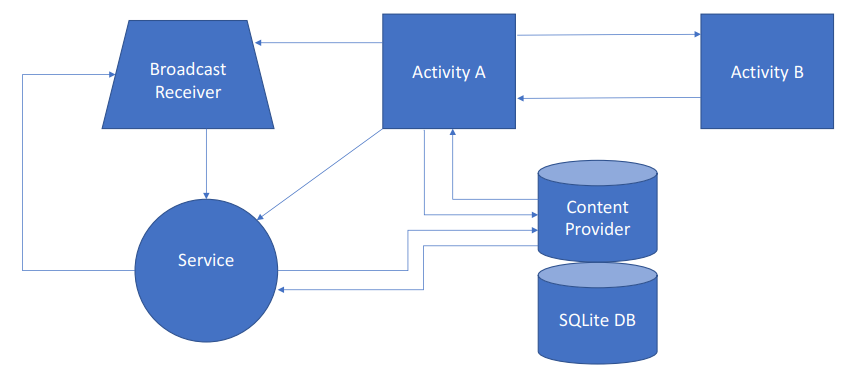
\includegraphics[scale=0.5]{broadcast.png}
\end{center}


\pagebreak
\section*{Reference section} \label{sec:reference}
\begin{description}
	\item[placeholder] \hfill \\
\end{description}
\end{document}
